% Seminar Information Retrieval Philipp Schalcher
% Betreuer: Ruxandra Domenig
% Thema: Evaluierung der Retrieval-Leistung einer Search Engine am Beispiel einer privaten MP3-Sammlung

\documentclass[12pt,a4paper,ngerman]{report}
\setlength{\parindent}{0pt}
\usepackage[ngerman]{babel}
\usepackage[utf8]{inputenc}
\usepackage{a4wide}
\usepackage{graphicx}
\usepackage{url}
\usepackage[final]{listings}
\usepackage{color}
\usepackage{amsmath}
\author{Philipp Schalcher}
\title{Evaluierung der Retrieval-Leistung einer Search Engine am Beispiel einer privaten MP3-Sammlung}
\date{\today}

\begin{document}
%\maketitle
\begin{titlepage}
\begin{center}

\includegraphics[width=0.25\textwidth]{img/zhaw.png}\\[0.5cm]
\textsc{\Large Zürcher Hochschule für Angewandte Wissenschaften}\\[1.0cm]
\textsc{\Large Seminar Concurrent Programming}\\[1.5cm]

% Title
\hrulefill \\[0.5cm]
{\huge \bfseries File-Server in C anhand CRUDL}\\[0.4cm]
\hrulefill \\[0.5cm]
%Author und Betreuer
\begin{minipage}{0.4\textwidth}
\begin{flushleft}
\emph{Author:}\\
Philipp \textsc{Schalcher}
\end{flushleft}
\end{minipage}
\begin{minipage}{0.4\textwidth}
\begin{flushright}
\emph{Betreuer:}\\
Nicolas \textsc{Schottelius}
\end{flushright}
\end{minipage}

\vfill

%Datum
{\large \today}

\end{center}
\end{titlepage}
\chapter*{Danksagung}
\tableofcontents
\begin{abstract}

\end{abstract}
\chapter*{Einleitung}
Ein wichtiger Teil der Systemprogrammierung ist das Concurrent Programming. Dabei steht nicht die Parallelisierung im Vordergrund, sondern das Problem, von Zugriffen auf Ressourcen und die damit auftretenden Schwierigkeiten. Gleichzeitige Bearbeitungen von Ressourcen können, je nach ausgeführter Arbeit, zu schwerwiegenden Problemen führen. Wird zum Beispiel eine Datei gelöscht, obwohl die Datei momentan an einem anderen Ort geöffnet ist und das System dies nicht bemerkt, tritt ein Konflikt auf. Soll die Datei nun gelöscht werden und der Bearbeiter verliert den Zugriff, oder soll die Datei einfach nicht gelöscht werden, mit dem Vermerk, dass die Datei geöffnet ist?
\\
In dieser Arbeit soll nun ein Dateiserver in C programmiert werden, der genau solche Probleme abfangen soll. Dabei gilt, dass der Server nach dem Schema CRUDL funktionieren soll. CRUDL steht für:
\begin{itemize}
	\item CREATE
	\item READ
	\item UPDATE
	\item DELETE
	\item LIST
\end{itemize}
Je nach aufgerufenem Task, darf eine Datei nicht mehr zugreifbar sein.
\\
\\
Die Arbeit soll keine realen Dateien verarbeiten können. Das Ziel liegt in der Realisierung des CRUDL-Systems. Die Dateien selber werden in einem Shared-Memory gespeichert (nur die Dateinamen). Sobald der Server gestoppt wird, gehen die Dateien im Shared-Memory verloren.
\chapter{Anleitung}
Der Server kann über die Binary \textquotedblleft run\textquotedblright gestartet werden. Im Konsolenfenster werden Nachrichten zur Initialisierung ausgegeben. Sobald der Server gestartet ist, kann über das Binary \textquotedblleft test\textquotedblright ein Testclient gestartet werden. Über diesen können Befehle an den Server gesendet werden.
\section{Befehle}
Der Server erkennt folgende Befehle:
\begin{itemize}
	\item CREATE Dateiname Grösse
	\item READ Dateiname
	\item UPDATE Dateiname Grösse
	\item DELETE Dateiname
	\item LIST
\end{itemize}

\section{CREATE}
Syntax: CREATE \textit{Dateiname} \textit{Grösse} \\
CREATE erstellt eine neue Datei im Fileserver. Als Parameter wird der gewünschte Dateiname und die Grösse als Zahl mitgegeben. Falls die Datei schon vorhanden ist, gibt der Server ein \textquotedblleft FILEEXISTS\textquotedblright zurück. Andernfalls wird bei Erfolg die Nachricht \textquotedblleft FILECREATED\textquotedblright an den Client gesendet.\\
\\
Beispiel: CREATE meineErsteDatei 30
\section{READ}
Syntax: READ \textit{Dateiname}
READ liest den Inhalt einer Datei aus und sendet sie an den Client. Falls der Dateiname nicht existiert, wird die Nachricht \textquotedblleft NOSUCHFILE\textquotedblright zurückgegeben.\\
\\
Beispiel: READ meineErsteDatei
\section{UPDATE}
Syntax: UPDATE \textit{Dateiname} \textit{Grösse}\\
Mit UPDATE wird die vorhandene Datei geändert. Dabei wird die Grösse und der Inhalt verändert. Existiert der angegebene Dateiname nicht, wird die Nachricht \textquotedblleft NOSUCHFILE\textquotedblright zurückgegeben. Ist der Befehl erfolgreich wird in einem zweiten Schritt der Inhalt verlangt.\\
\\
Beispiel: UPDATE meineErsteDatei 13
\section{DELETE}
Syntax: DELETE \textit{Dateiname}\\
Nach dem Aufruf von DELETE wird die ausgewählte Datei gelöscht. Dabei gibt der Befehl die Meldung \textquotedblleft NOSUCHFILE\textquotedblright zurück, falls kein Eintrag mit dem Dateinamen bekannt ist. Ansonsten erhält man die Nachricht \textquotedblleft DELETED\textquotedblright . \\
\\
Beispiel: DELETE meineErsteDatei
\section{LIST}
Syntax: LIST
LIST veranlasst den Server dazu, alle Dateien zu zählen und deren Namen an den Client zu senden.
\section{Beschränkung}
Durch den Einsatz der Semaphore ist der Server momentan auf maximal 10 gleichzeitige Read-Vorgänge eingeschränkt. Dies könnte mit grösseren Semaphor verändert werden. Da aber keine Angaben im Auftrag gemacht wurden, werde ich die Einstellung in diesem Zustand belassen.
\chapter{Ausgangslage}
Auf Wunsch des Dozenten in Concurrent Programming soll entweder ein Datei-Server oder ein Mehrbenutzereditor in C programmiert werden. Diese Arbeit behandelt die Aufgabe mit dem Datei-Server. Dabei muss der Server gewisse Bedingungen erfüllen. Diese wären:
\begin{itemize}
	\item Keine SEGV während des Betriebs.
	\item Jeder Client der verbindet, soll mit einem eigenen Prozess behandelt werden.
	\item Server muss nach CRUDL arbeiten.
	\item Das echte Dateisystem darf nicht genutzt werden.
	\item Dateien sind nur im Speicher vorhanden.
\end{itemize}

CRUDL bedeutet soviel wie CREATE, READ, UPDATE, DELETE und LIST. Diese 5 Befehle müssen vom Server umgesetzt werden. Der Fokus liegt dabei auf den Zugriff von verschiedenen Prozessen auf Dateien (als Ressourcen). Gewisse Operationen wie DELETE müssen Dateien komplett sperren, damit diese während der Operationen nicht von anderen Operationen besetzt werden können. Das heisst, während eines DELETE darf kein READ, UPDATE oder LIST durchgeführt werden. Innerhalb dieser Befehle gibt es mehrere Kombinationen solcher Sperrungen. Diese müssen abgefangen werden.
\section{Lösungsansatz}
Die Problematik besteht für mich aus 3 Teilproblemen. Das erste Problem ist die Netzwerkverbindung und die darauf folgende Erstellung eines neuen Prozesses, der die Anfragen annimmt und verarbeitet. Als Lösung würde ich daher auf eine normale TCP/IP Verbindung setzen. Diese wird über Sockets gelöst. Sobald ein Client verbindet, wird per fork() ein neuer Prozess erstellt, der als Child-Prozess die Anfragen des Clients annimmt und bearbeitet. Innerhalb des Child-Prozesses müssen daher die Befehle abgefangen werden und die eigentlichen Aktionen ausgeführt werden.
\\
Als zweites Problem sehe ich die Speicherung der "Dateien". Hier würde ich so vorgehen, indem ich eine Struktur aufbaue, die für jede Datei ihren Dateinamen, ihre Grösse und den Inhalt speichert. eine einzelne Struktur soll also eine Datei symbolisieren. Um mehrere Dateien speichern zu können, wird aus der Struktur ein Array erstellt. Allerdings begrenzt ein Array die Anzahl der zu verarbeitenden Dateien. Allerdings könnte dies gleichgesetzt werden mit dem Plattenspeicher, der irgendwann auch voll ist.
\\
Als drittes Problem ist die Sperrung der Dateien ein zentraler Punkt. Da für den Server keine globalen Sperren genutzt werden dürfen, würde ich Semaphore einsetzen, die die einzelnen Codeteile sperren und so von Prozessen nicht gleichzeitig ausgeführt werden können. Der Semaphor an sich muss aber mehr als ein "Ticket" vergeben können, da zum Beispiel READ mehrfach ausgeführt werden darf. Allerdings muss ein DELETE den kompletten Semaphor besetzen, damit keine anderen Operationen durchgeführt werden können.
Auch hier gilt wieder, das mit der Semaphorengrösse auch die Anzahl Clients beschränkt wird. So können bei einem Semaphor mit 10 Tickets maximal 10 Clients gleichzeitig einen READ durchführen. Auch wenn 20 Clients verbunden wären, so würden doch immer nur 10 bedient werden.
\chapter{Realisierung}
In diesem Kapitel werde ich auf die Realisierung eingehen. Ein kurzer Abschnitt handelt von meiner Vorgehensweise und wie ich den Server aufgebaut habe. Schwerpunkt wird allerdings auf den Bereich \textquotedblleft Schwierigkeiten\textquotedblright und \textquotedblleft Testing\textquotedblright gelegt.
\section{Implementation}
Der ganze Server ist in einem C-Sourcefile zu finden. Der Aufbau ist relativ einfach:
\begin{itemize}
	\item Includes der Bibliotheken
	\item Globale Variablen definieren
	\item Funktionen definieren
	\item Main-Funktion definition
		\begin{itemize}
		\item Erstellung des Signal-Handler
		\item Erstellung des Shared-Memory
		\item Erstellung des Semaphore
		\item Aufbau des Netzwerkteils
		\item Abfangen von Verbindungsanfragen und Prozesserstellung
			\begin{itemize}
			\item Abfangen des LIST-Befehls
			\item Abfangen des CREATE-Befehls
			\item Abfangen des READ-Befehls
			\item Abfangen des UPDATE-Befehls
			\item Abfangen des DELETE-Befehls
			\end{itemize}
		\end{itemize}
\end{itemize}
Die komplette Logik ist in den Bereichen der Befehlsabfragen zu finden. Die Dateien werden in einer definierten Struktur gespeichert, welche als Array auf das Shared-Memory gelegt wird. Sobald ein freier Platz oder eine bestimmte Datei gesucht werden muss, durchläuft das Array eine Schlaufe bis die Länge des String im Namen gleich 0 ist. So wissen wir, dass wir die letzte Position erreicht haben. Wie die Befehle genau implementiert sind, wird in den folgenden Abschnitten erklärt.
\subsection{Implementation LIST}
Für den Befehl List, wird das Array durchgelaufen und die Anzahl gefundenen Dateien gezählt. Da auch Einträge mit Namen \textquotedblleft EMPTY\textquotedblright vorkommen können (mehr dazu im Kapitel \textquotedblleft Implementation DELETE\textquotedblright), werden diese ignoriert. Die korrekten Dateinamen werden an einen vorhanden String angehängt. Ist die letzte Position im Array erreicht, wird die Nachricht generiert und an den Client gesendet. Danach steht der Server wieder für die nächste Eingabe zur Verfügung.
\subsection{Implementation CREATE}
Das Array wird wieder durchgegangen bis das Ende erreicht ist (wieder über die Längenprüfung von Name) oder ein Eintrag mit \textquotedblleft EMPTY\textquotedblright gefunden wird. Ist der vorgegebene Dateiname schon vorhanden, bricht der Vorgang ab. Ansonsten wird der Name, die Grösse, der Semaphorwert gesetzt und der Client wird nach dem Inhalt gefragt. Der Client muss den Inhalt eingeben, welcher dann im Feld Content gespeichert wird.
\subsection{Implementation READ}
Das Array wird nach dem angegebenen Namen durchsucht. Wird kein Eintrag gefunden, erhält man ein \textquotedblleft NOSUCHFILE\textquotedblright . Ansonsten holt sich der Prozess ein Semaphorticket und liest den Inhalt. Der Inhalt wird dann an den Client gesendet. Zum Abschluss gibt der Prozess das Semaphorticket wieder zurück. Sind alle Tickets verbraucht, wartet der Prozess bis eines frei wird.
\subsection{Implementation UPDATE}
Der erste Teil ist gleich wie im READ-Bereich. Ist das spezifische File gefunden, werden zuerst alle Semaphortickets reserviert, dann die Grösse und der Inhalt auf Leer geändert. Der Server fragt danach wieder den Client an, um den Inhalt zu erhalten. Sobald der Client den Inhalt generiert hat und zurückgegeben wurde, speichert der Server die Werte im Feld Content. Danach werden die Semaphortickets zurückgegeben. Solange UPDATE aktiv ist, kann kein READ, DELETE oder UPDATE durchgeführt werden.
\subsection{Implementation DELETE}
Falls bei einem Löschvorgang der Name auf NULL gesetzt wird, erhält das Array einen zweiten Punkt, wo die Stringlänge ebenfalls gleich 0 ist. Daraus folgt, dass das Array nicht mehr komplett durchgelaufen werden kann. Daher wird der Name nur auf \textquotedblleft EMPTY\textquotedblright gesetzt. So ist garantiert, dass das Array immer komplett durchgelaufen werden kann. Die restlichen Einträge werden auf NULL, 0 oder leer gesetzt.
\subsection{Implementation Semaphor}
Im Array enthält jeder Eintrag eine Variable semval. Diese beinhaltet die maximalen Tickets für eine Datei. In den einzelnen Befehlsbereichen wird bei der Ausführung der Wert ausgelesen und per semctl in den Semaphor geladen. Danach holt sich der Prozess ein oder alle Tickets per semop. Sobald der kritische Bereich ausgeführt ist, wird das reservierte Ticket frei gegeben.
\begin{figure}[h!]
\centering
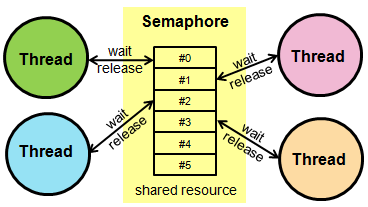
\includegraphics[width=10cm]{img/semaphore.png}
\caption{Semaphor sperrt Ressource für Threads\protect\footnotemark}
\end{figure}
\footnotetext{Quelle: \url{http://www.mbed.org}}
\section{Schwierigkeiten}
In diesem Abschnitt möchte ich auf einige Probleme eingehen, die bei der Erstellung des Servers aufgetreten sind. Im Anschluss zu den jeweiligen Problemen wird meine Lösung angegeben.
\subsection{Struktur Datei}
In der Struktur Datei werden die Informationen zu den Dateien gespeichert. Hier gab es 2 grosse Entscheidungen bei der Implementation. Das erste Problem bestand in der Definition von der Variable Name und Content. Sind diese als undefinierte Arrays von Chars deklariert, zeigt der nächste Eintrag im Strukturarray auf den gleichen Speicher, wie der vordere. So entstand das Problem, dass ein zweiter Eintrag den Namen des ersten Eintrages änderte. Dies ging so weiter für jeden weiteren Eintrag in der Struktur.\\
\\
Das zweite Problem lag beim Durchsuchen. Der Name im Array wurde als Referenz genutzt. Der Durchlauf per Schlaufe lief mit der Prüfung auf NULL aber nur schlecht durch. Auch funktionierte er teilweise nicht, so dass das Programm hängen blieb und nicht mehr reagieren konnte.
\subsubsection{Lösung}
Problem 1 kam aus der Eigenschaft des undefiniertem Array. Der Speicher des Namensvariable zeigt für alle Einträge im Strukturarray auf die gleiche Adresse. So entstand die Eigenschaft, dass jeder weitere Eintrag den Namen auf die vorhergehenden Einträge vererbte. Die Lösung war, dass der Name nicht mehr eine undefinierte Länge besitzt, sondern das Char-Array von Beginn an auf eine bestimmte Grösse definiert wurde.\\
\\
Problem 2 lies den Server an einer bestimmten Stelle einfrieren. Dieser Effekt war aber nicht voraussagbar, da er nur sporadisch auftrat. Die Änderung der while-Schleife auf die Prüfung der Stringlänge behob dieses Problem. 
\subsection{Generierung Messages}
Es trat das Problem auf, dass bei die Rückmeldungen (besonders bei der Funktion LIST) nicht korrekt in die Stringvariable geschrieben wurde. Im schlimmsten Fall blieb der Server an einem bestimmten Punkt bei der Ausführung stecken.
\subsubsection{Lösung}
Zwei verschiedene Lösungen hatten sich bei der Implementierung angeboten. Da der Inhalt meistens mit strcpy oder strcat gebaut werden, lag das Problem bei der Vorbereitung des Speichers. Bei der ersten Variante setzte ich für die Speicherreservierung ein malloc() ein. Allerdings funktionierte diese Lösung nur begrenzt. Die Nachricht wurde, aufgrund der Grösse bei mehreren Dateien, nicht mehr anzeigbar. Die letzten Dateien wurden nicht mehr in den String eingefügt. Anpassen der Grösse bei malloc() hat leider nicht zum gewünschte Erfolg geführt. So stellte ich die Nachrichtenvariable auf eine feste Grösse um. So wurde der Speicher reserviert und alle Dateien konnten angezeigt werden. Je nach Grösse der Dateiliste kann auch hier dieses Problem wieder auftauchen.
\newpage
\subsection{Semaphore und Dateien}
Da die Semaphorwerte in der Struktur der Datei gespeichert werden und für jede Operation ausgelesen werden muss, wird auch immer der Befehl semctl() ausgeführt. So entstand das Problem, dass bei mehrfachen Zugriff die Werte immer wieder zurückgesetzt wurde. So hatte der Semaphor den Wert 10 beim Start, nach dem ersten semop() des UPDATES wurde er 0. Ein READ-Befehl setzte hingegen den Wert des Semaphors wieder auf 10. So sperrte zwar der Semaphor, wurde aber automatisch erhöht und dadurch umgangen.
\subsubsection{Lösung}
Der Wert aus dem Semaphor soll wieder zurück in die Datei geschrieben werden. Der Wert der Variable ändert sich während der Laufzeit und passt sich an. Werden 10 Plätze reserviert, so steht in der Variable in der Struktur auch der Wert 0 danach. Ein zweiter Prozess liesst diese vor semctl() aus und erhält so den aktuellen Semaphorwert. Einzelne Dateien werden so gesperrt, ohne dass andere Dateien beeinträchtigt sind.
\section{Testing}
Das Testing wurde während des Entwicklungsprozesses in den Fokus gelegt. Die Tests wurden manuell durchgeführt mit dem Binary test. Das Binary wechselt ausschliesslich zwischen read() und write() per TCP. Der Server musste sich dementsprechend anpassen.
\subsection{Test 1: Netzwerk}
Der erste Test kümmerte sich nur um die Verbindung zum Server. Er war erfolgreich, sobald ein Client (test) verbinden konnte. Dies klappte reibungslos.
\subsection{Test 2: Fork}
Der zweite Test überprüfte das Handling von mehreren Clients. Nachdem der fork() in den Server eingebaut wurde, testete ich mit 4 Clients einen gleichzeitigen Zugriff. Dies funktionierte und die Prozesse des Servers kümmerten sich um die Clients.
\subsection{Test 3: Befehlsabfrage}
Durch strtok wird der übermittelte String aufgeteilt. So konnte ich vergleichen, welchen Befehl der User abgesetzt hat. Der Test lief daraus hinaus, dass bei der erfolgreichen Erkennung eine Nachricht ausgegeben wurde.
\subsection{Test 4: Dateioperationen}
Nach der Implementation der Befehle testete ich die einzelnen Befehle mit dem Client. Dabei galt, dass mehrere Dateien erstellt (maximal 10 gestestet), gelesen, aktualisiert und gelöscht werden mussten. Dieser Test brauchte mehr Zeit, da immer wieder kleine Änderungen am Code vorgenommen werden mussten. Daher ging ich so vor, jeden Befehl einzeln zu implementieren, zu testen. Erst als die Befehle funktionierten, ging ich zum nächsten über. Als Letztes kümmerte ich mich um LIST. So konnte ich sicherstellen, dass die Befehle korrekt arbeiten.
\subsection{Test 5: Shared Memory}
Für diesen Test benutzte ich zwei Clients, die sich mit dem Server verbinden. Danach erstellte ich einige Dateien. Nun wechselte ich in den zweiten Client und verband mit dem Server. Mit dem Befehl LIST musste ich nun als erfolgreiches Ergebnis die Dateinamen erhalten. 
\subsection{Test 6: Semaphor}
Als letzten Test betrachtete ich die Sperrung der Dateien. Auch hier verband ich wieder zwei Clients mit dem Server und erstellte einige Dateien. Nun musste Client 1 ein UPDATE auf eine Datei ausführen. Da der Client nach dem Befehl den Inhalt verlangt, kann ich dadurch eine Datei auf unbestimmte Zeit sperren. Während Client 1 die Eingabe abwartete, versuchte ich ein READ im Client 2 auf die gleiche Datei auszuführen. Nach meiner Idee sollte nun beim READ nicht passieren, bis in Client 1 der Inhalt eingefügt wurde. Da ich nur mit UPDATE eine Sperre bauen konnte, habe ich die Schlussfolgerungen aus den Tests analog auf die restlichen Befehle übertragen.
\chapter{Fazit}
\end{document}